%! TEX root = main.tex

\begin{figure*}[!hbt]
    \centering%
    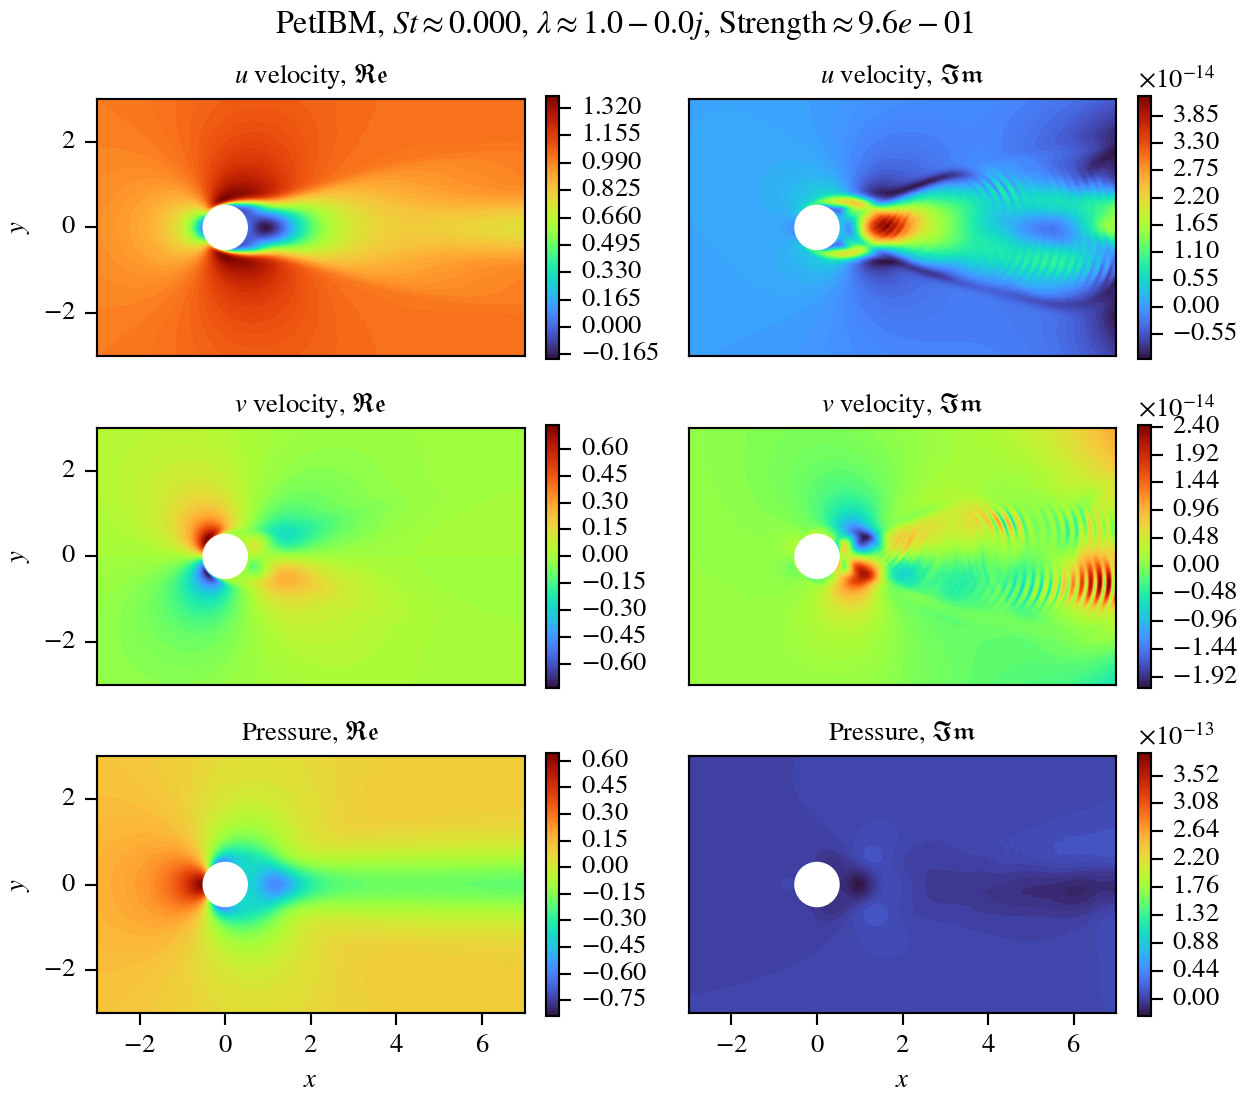
\includegraphics[width=0.95\textwidth]{cylinder-2d-re200/koopman_petibm_000_st0.000.png}%
    \caption{%
        The \num{1}st mode in PetIBM.
    }
    \label{fig:cylinder-re200-koopman-petibm-1st}%
\end{figure*}

\begin{figure*}[!hbt]
    \centering%
    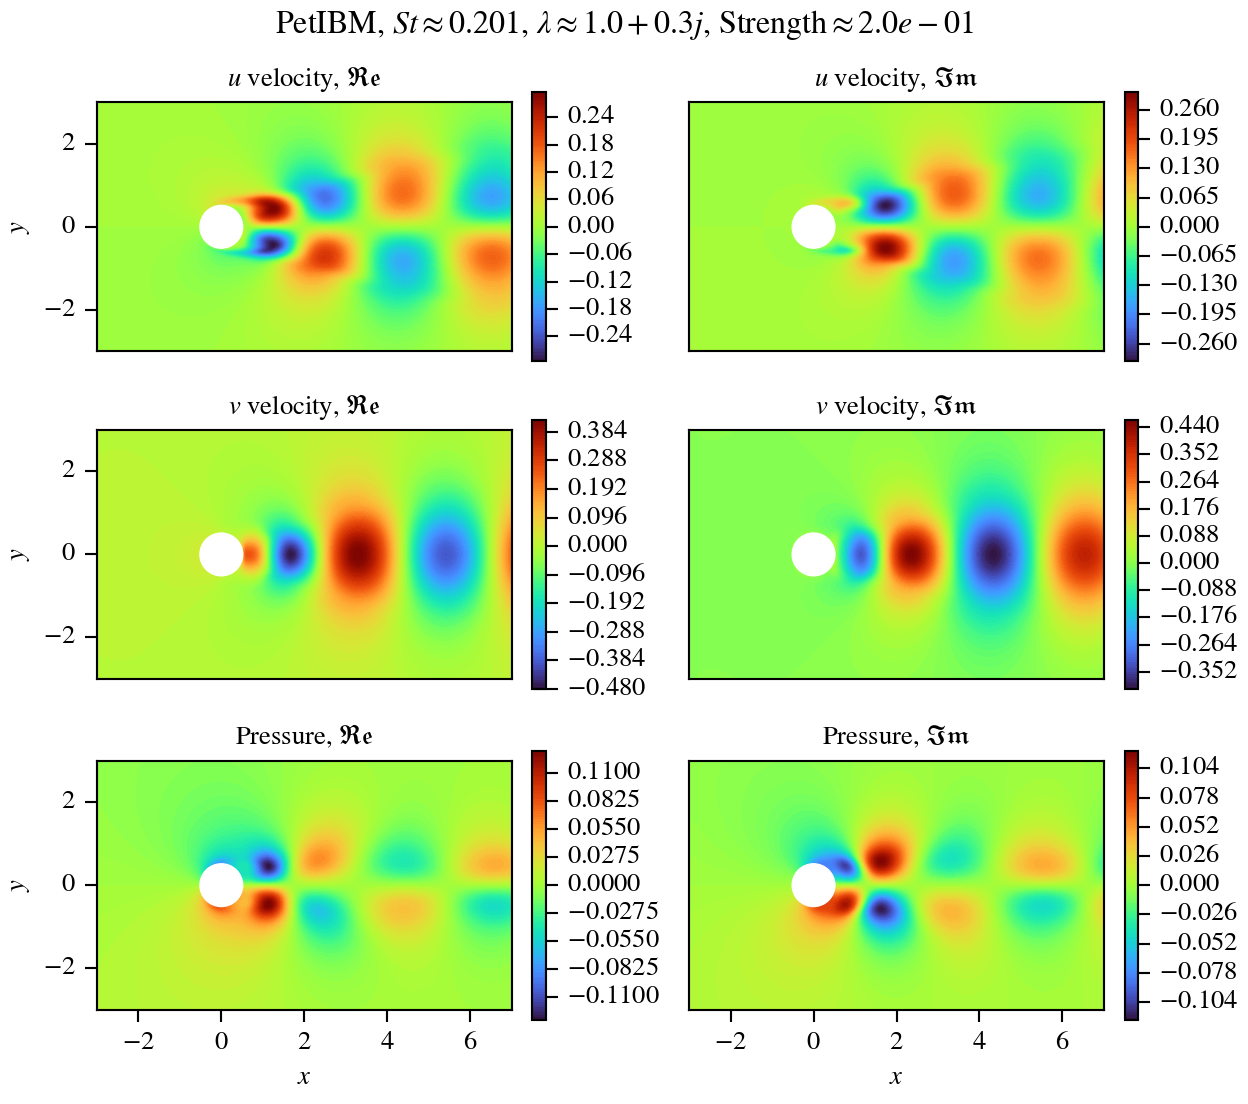
\includegraphics[width=0.95\textwidth]{cylinder-2d-re200/koopman_petibm_001_st0.201.png}%
    \caption{%
        The \num{2}nd mode in PetIBM.
    }
    \label{fig:cylinder-re200-koopman-petibm-2nd}%
\end{figure*}

\begin{figure*}[!hbt]
    \centering%
    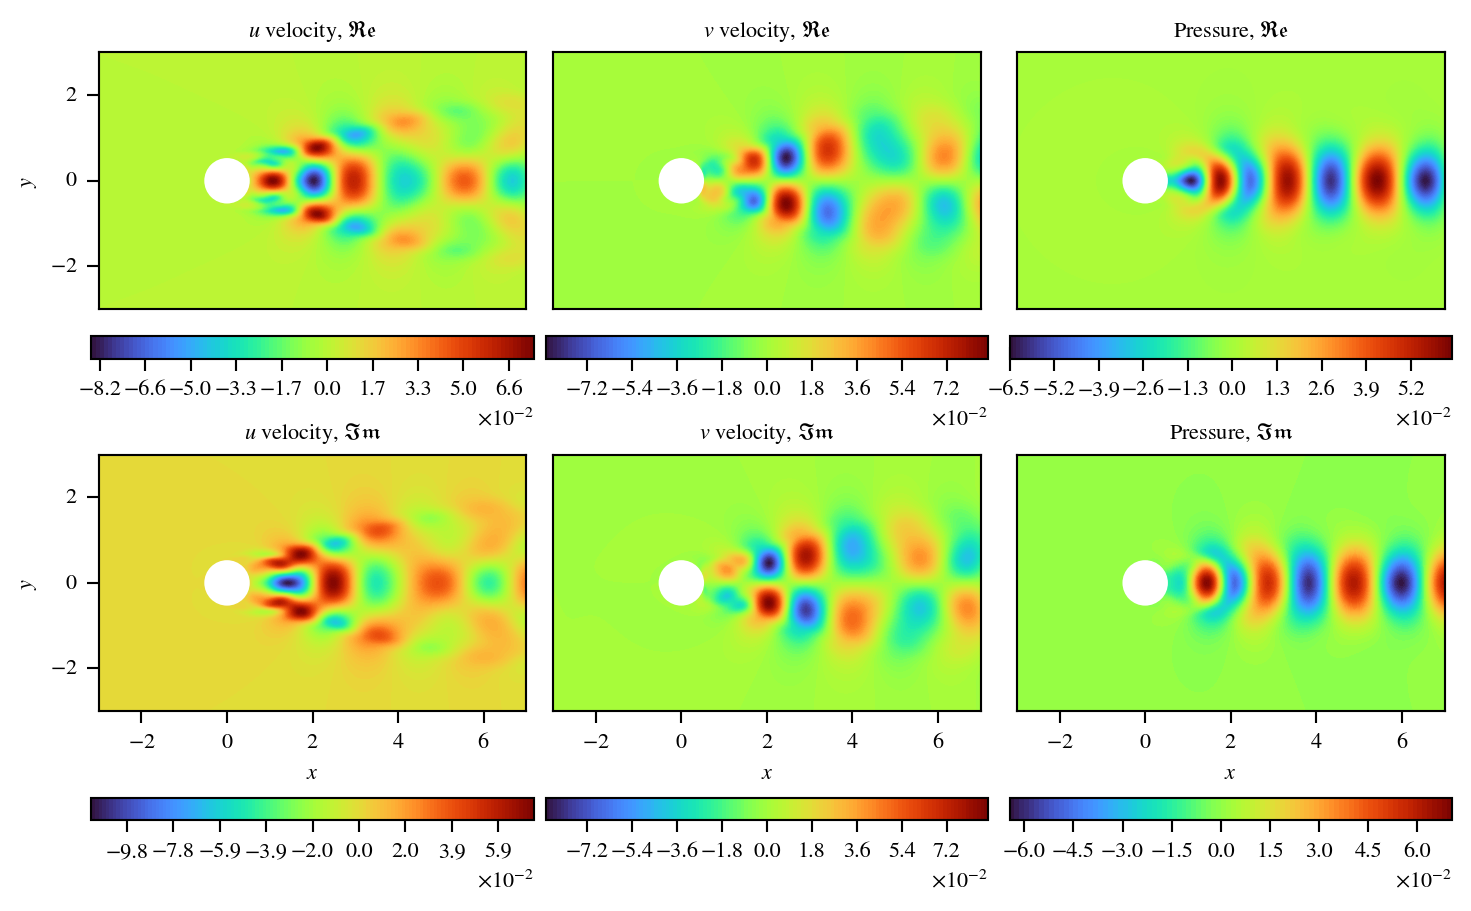
\includegraphics[width=0.95\textwidth]{cylinder-2d-re200/koopman_petibm_002_st0.403.png}%
    \caption{%
        The \num{3}rd mode in PetIBM.
    }
    \label{fig:cylinder-re200-koopman-petibm-3rd}%
\end{figure*}

\begin{figure*}[!hbt]
    \centering%
    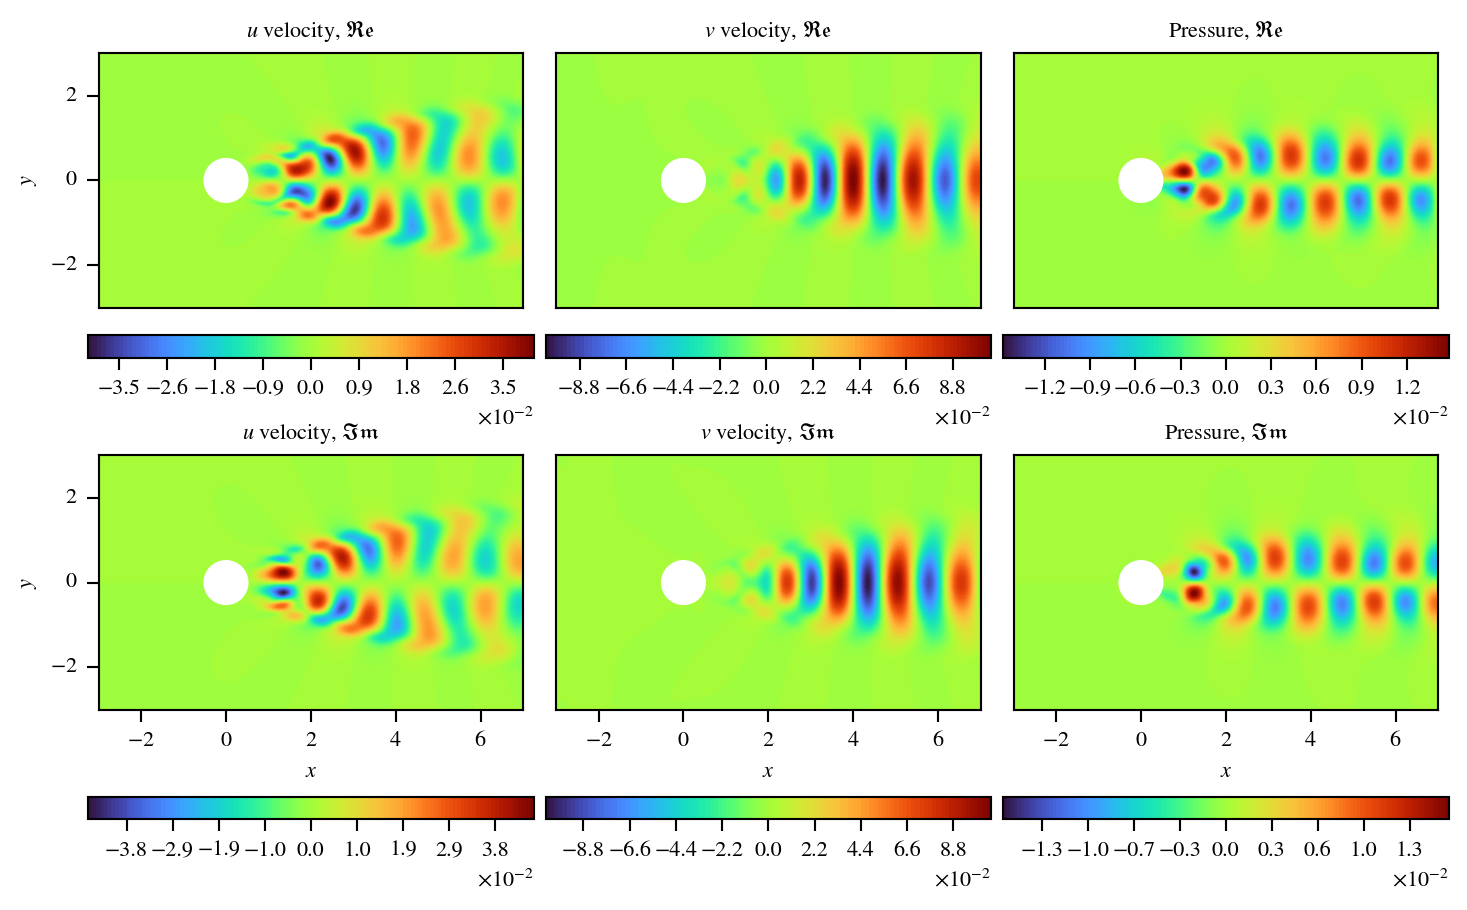
\includegraphics[width=0.95\textwidth]{cylinder-2d-re200/koopman_petibm_003_st0.604.png}%
    \caption{%
        The \num{4}th mode in PetIBM.
    }
    \label{fig:cylinder-re200-koopman-petibm-4th}%
\end{figure*}

\begin{figure*}[!hbt]
    \centering%
    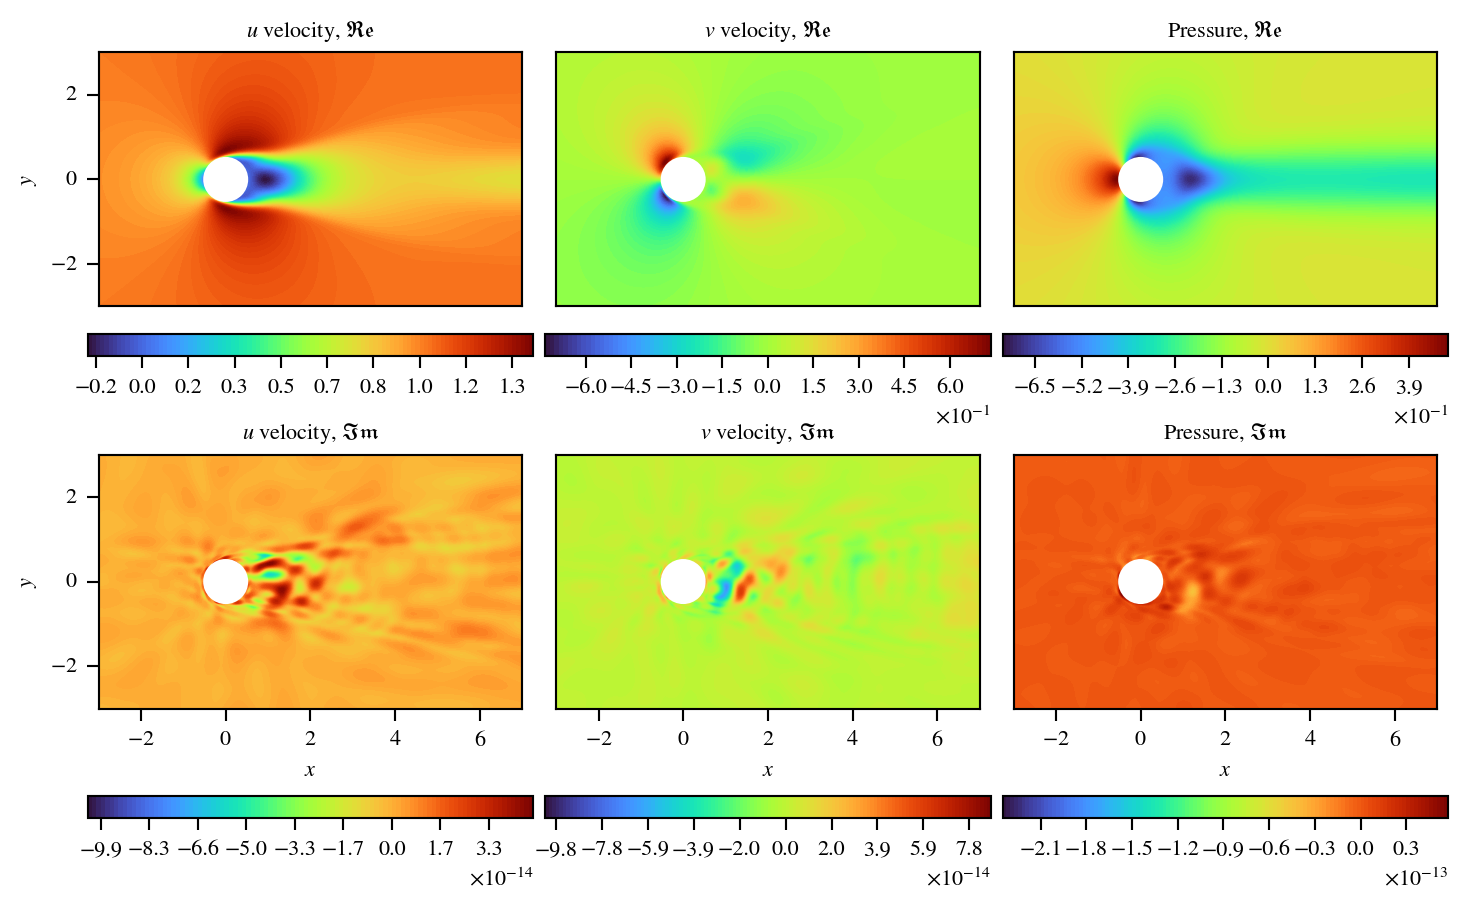
\includegraphics[width=0.95\textwidth]{cylinder-2d-re200/koopman_pinn_000_st0.000.png}%
    \caption{%
        The \num{1}st primary mode in data-driven PINN.
    }
    \label{fig:cylinder-re200-koopman-pinn-primary-1st}%
\end{figure*}

\begin{figure*}[!hbt]
    \centering%
    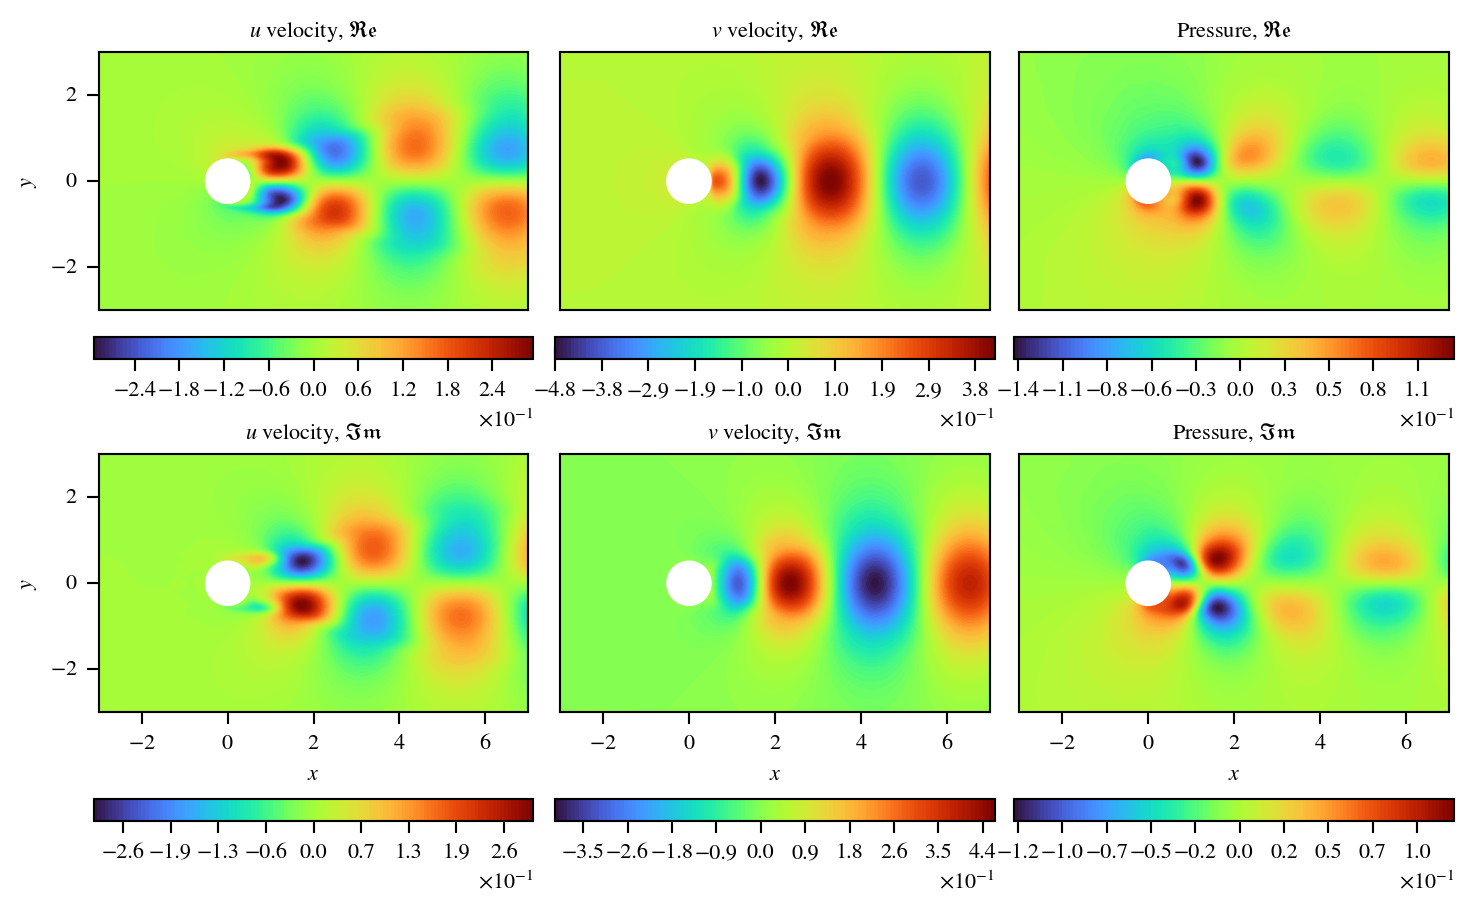
\includegraphics[width=0.95\textwidth]{cylinder-2d-re200/koopman_pinn_001_st0.201.png}%
    \caption{%
        The \num{2}nd primary mode in data-driven PINN.
    }
    \label{fig:cylinder-re200-koopman-pinn-primary-2nd}%
\end{figure*}

\begin{figure*}[!hbt]
    \centering%
    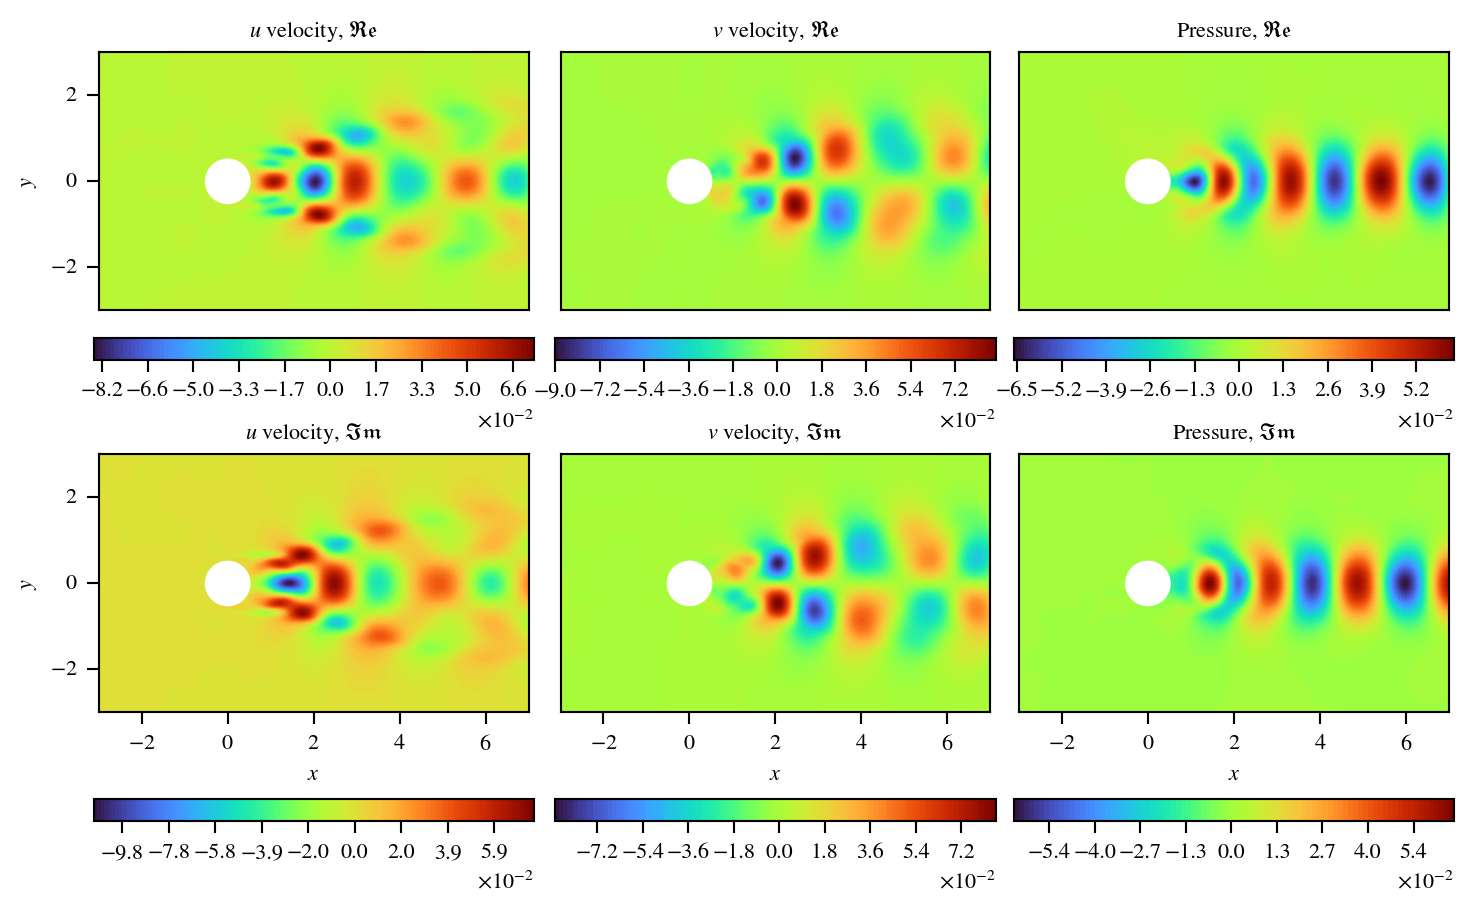
\includegraphics[width=0.95\textwidth]{cylinder-2d-re200/koopman_pinn_006_st0.403.png}%
    \caption{%
        The \num{3}rd primary mode in data-driven PINN.
    }
    \label{fig:cylinder-re200-koopman-pinn-primary-3rd}%
\end{figure*}

\begin{figure*}[!hbt]
    \centering%
    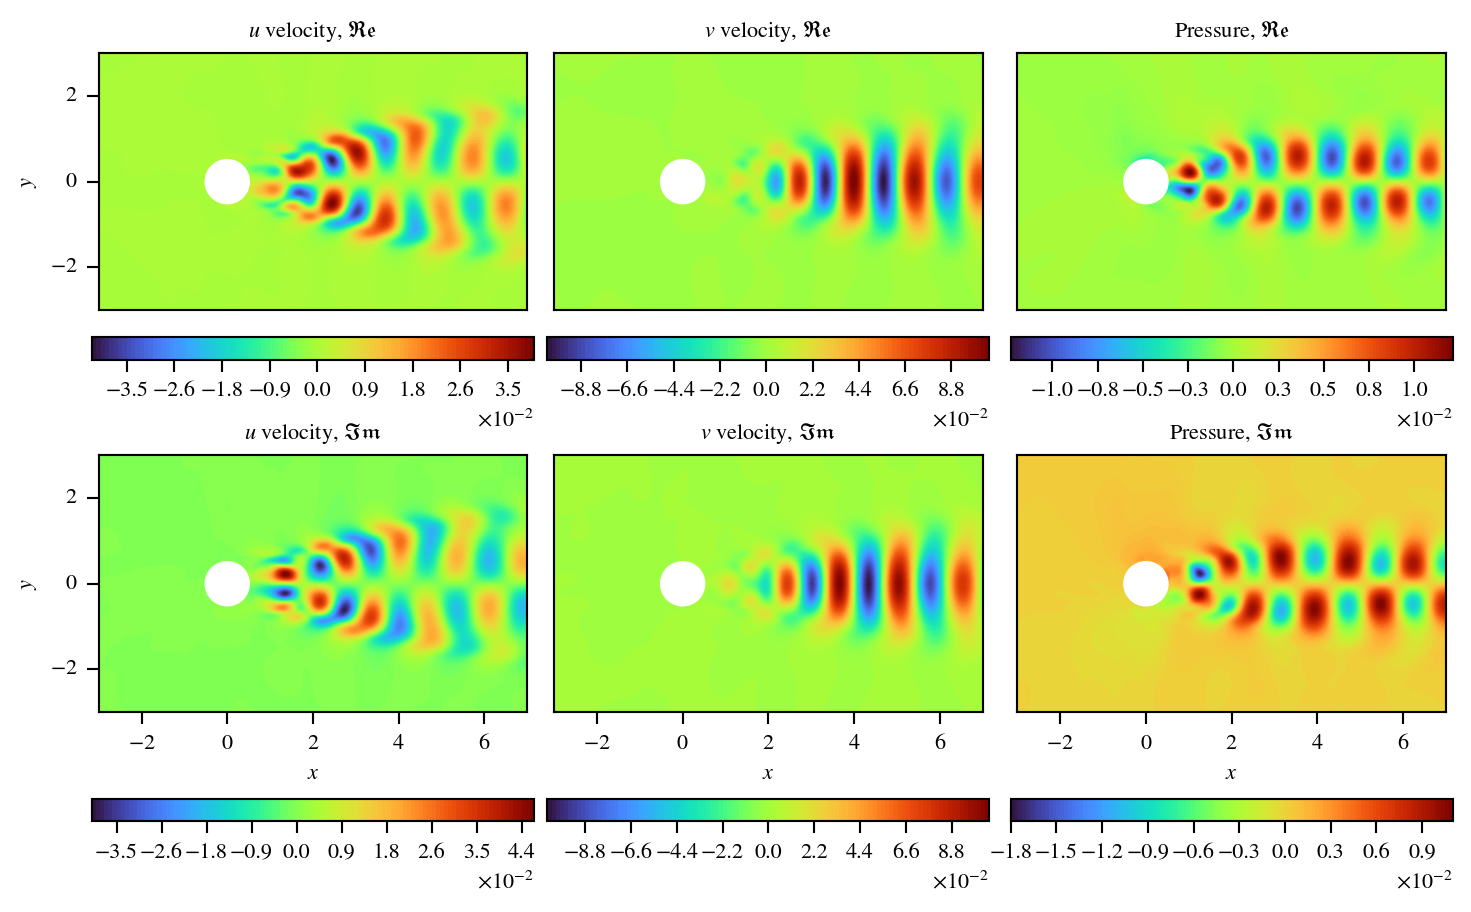
\includegraphics[width=0.95\textwidth]{cylinder-2d-re200/koopman_pinn_007_st0.604.png}%
    \caption{%
        The \num{4}th primary mode in data-driven PINN.
    }
    \label{fig:cylinder-re200-koopman-pinn-primary-4th}%
\end{figure*}

\begin{figure*}[!hbt]
    \centering%
    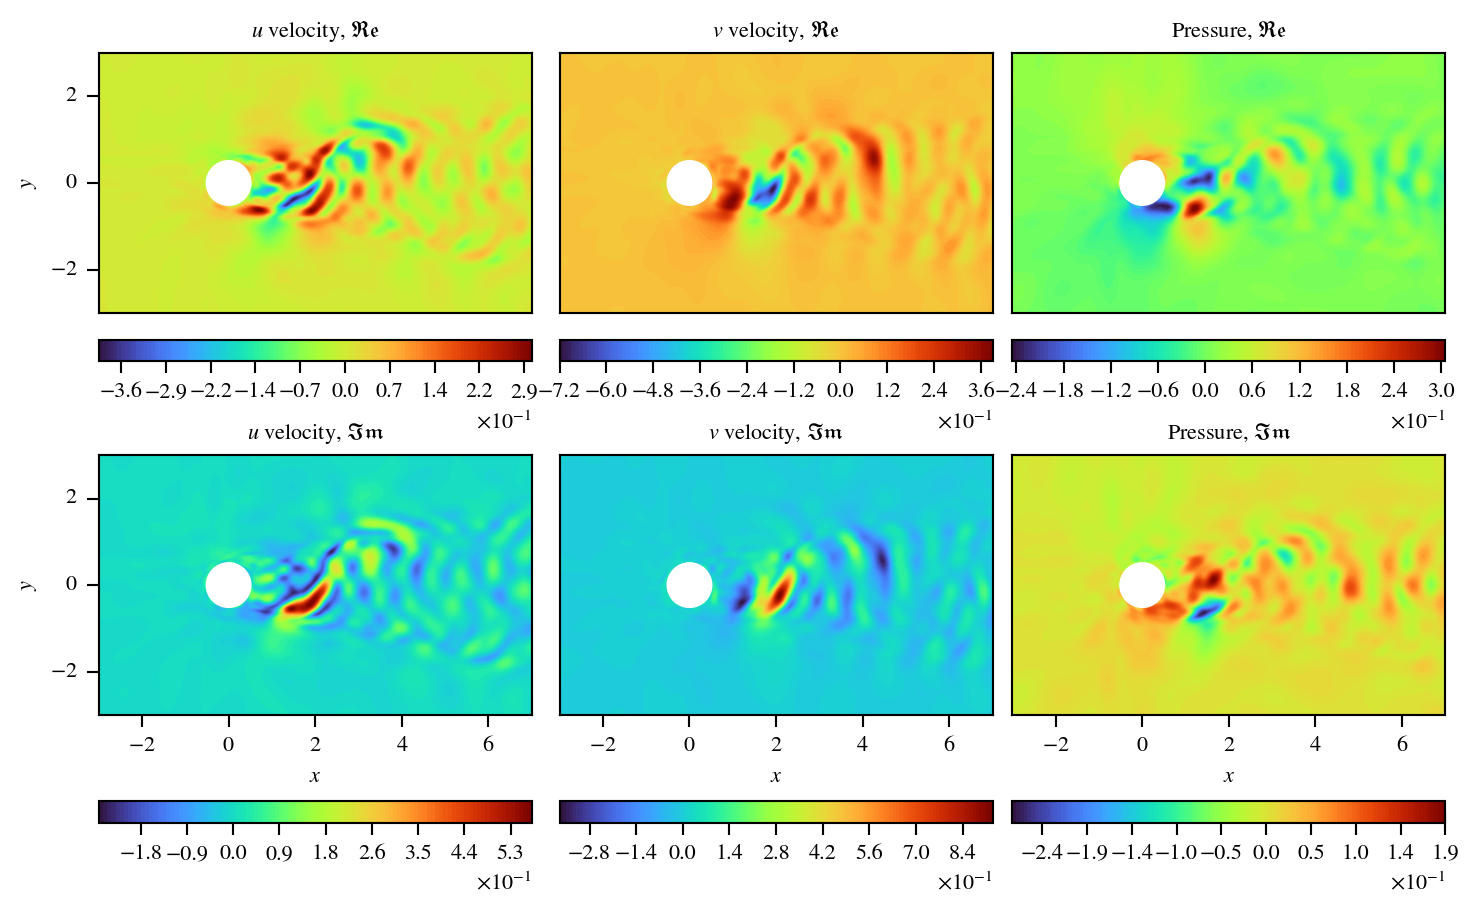
\includegraphics[width=0.95\textwidth]{cylinder-2d-re200/koopman_pinn_002_st1.142.png}%
    \caption{%
        The \num{1}st damped mode in data-driven PINN.
    }
    \label{fig:cylinder-re200-koopman-pinn-damped-1st}%
\end{figure*}

\begin{figure*}[!hbt]
    \centering%
    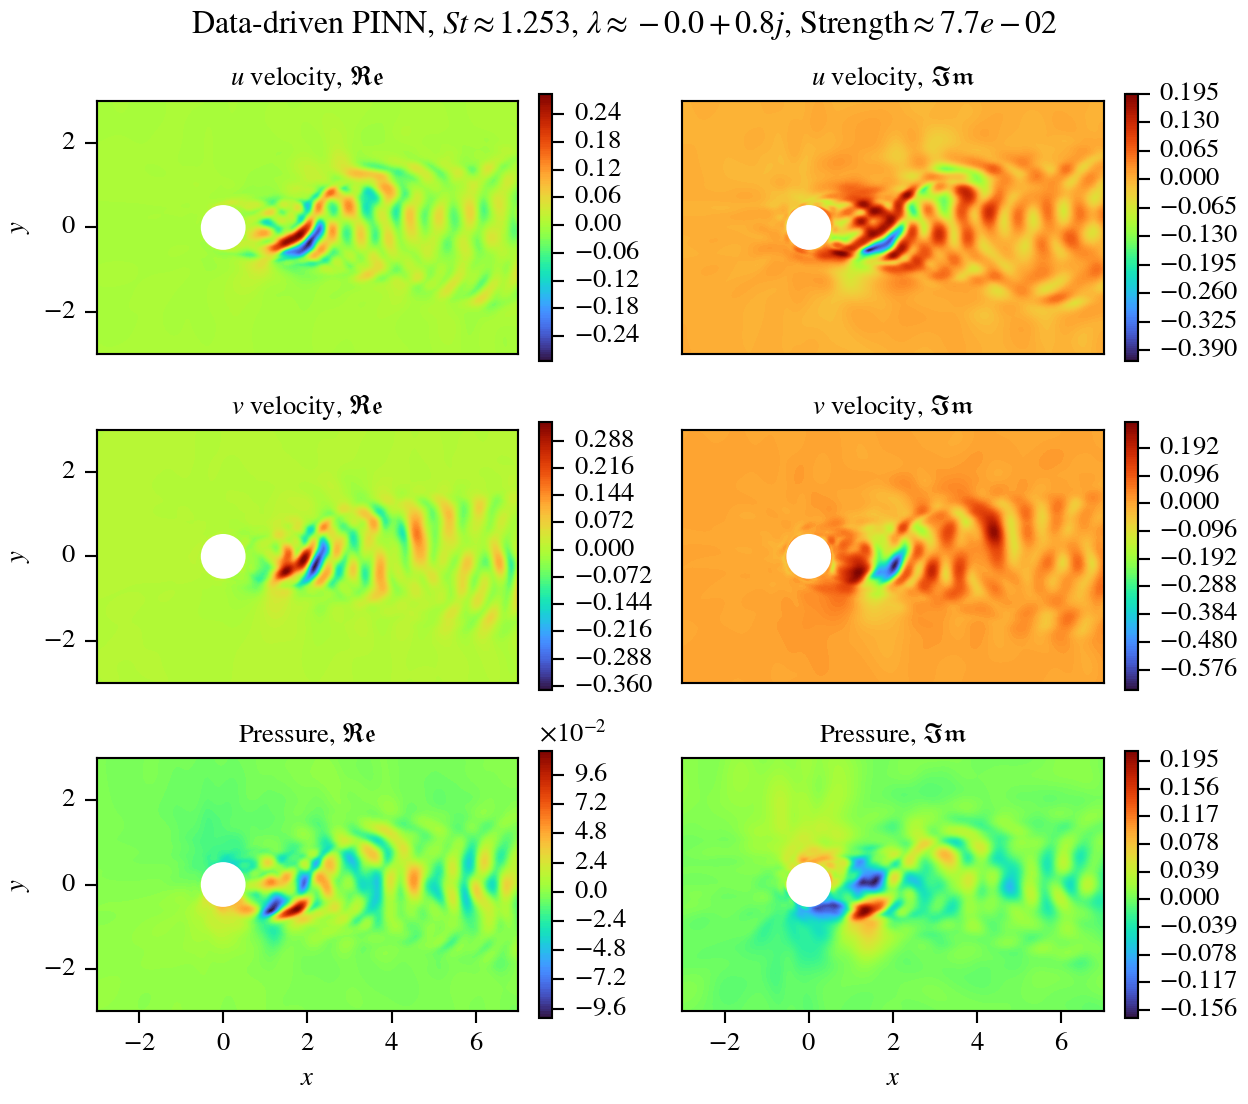
\includegraphics[width=0.95\textwidth]{cylinder-2d-re200/koopman_pinn_003_st1.253.png}%
    \caption{%
        The \num{2}nd damped mode in data-driven PINN.
    }
    \label{fig:cylinder-re200-koopman-pinn-damped-2nd}%
\end{figure*}

\begin{figure*}[!hbt]
    \centering%
    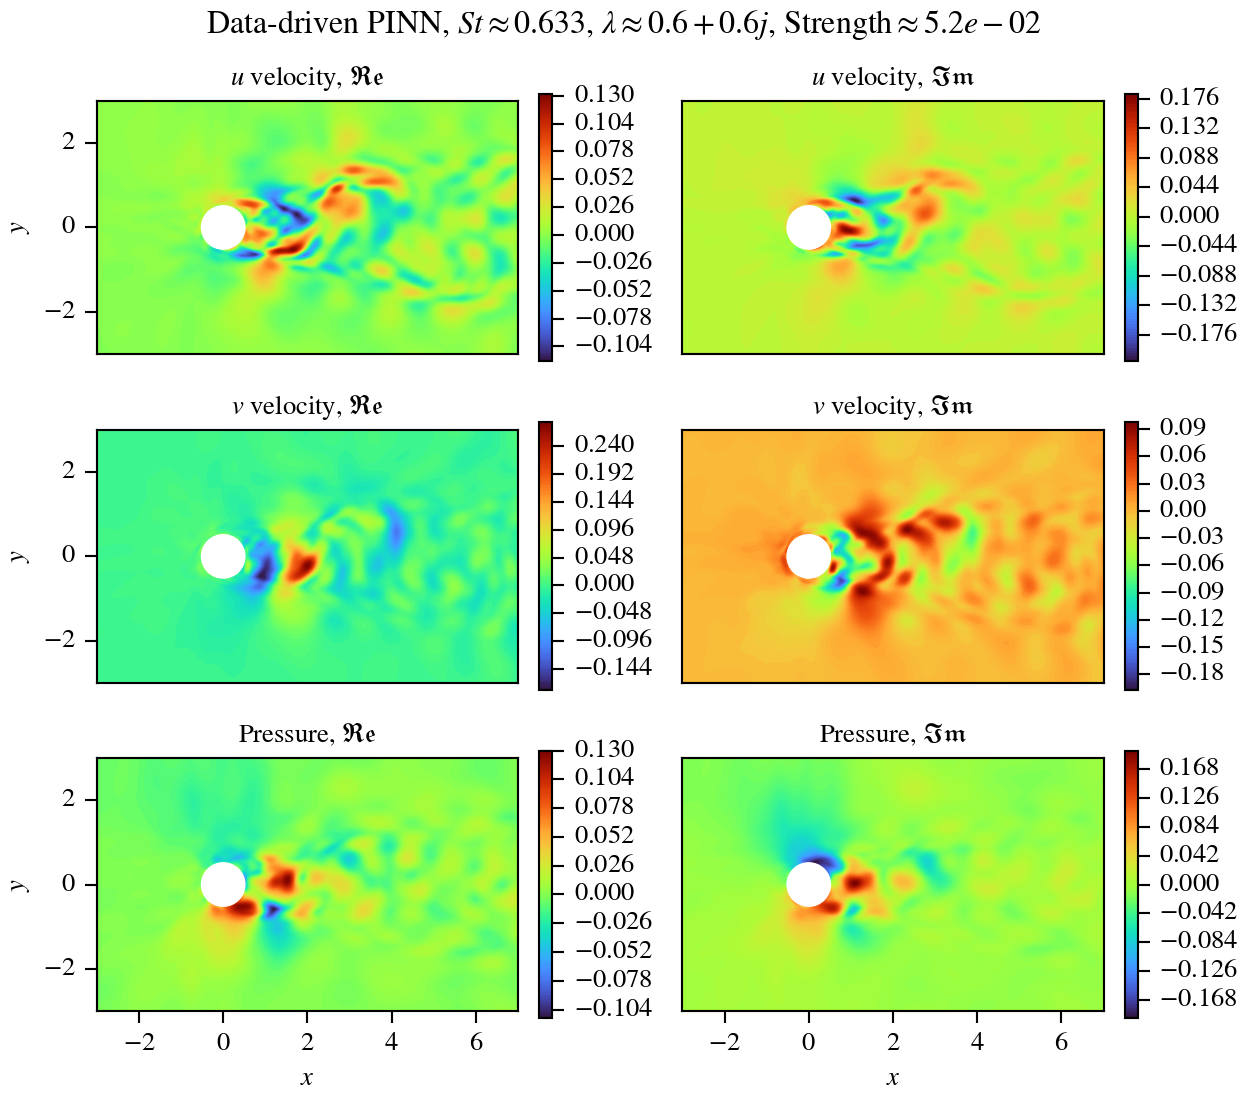
\includegraphics[width=0.95\textwidth]{cylinder-2d-re200/koopman_pinn_004_st0.633.png}%
    \caption{%
        The \num{3}rd damped mode in data-driven PINN.
    }
    \label{fig:cylinder-re200-koopman-pinn-damped-3rd}%
\end{figure*}

\begin{figure*}[!hbt]
    \centering%
    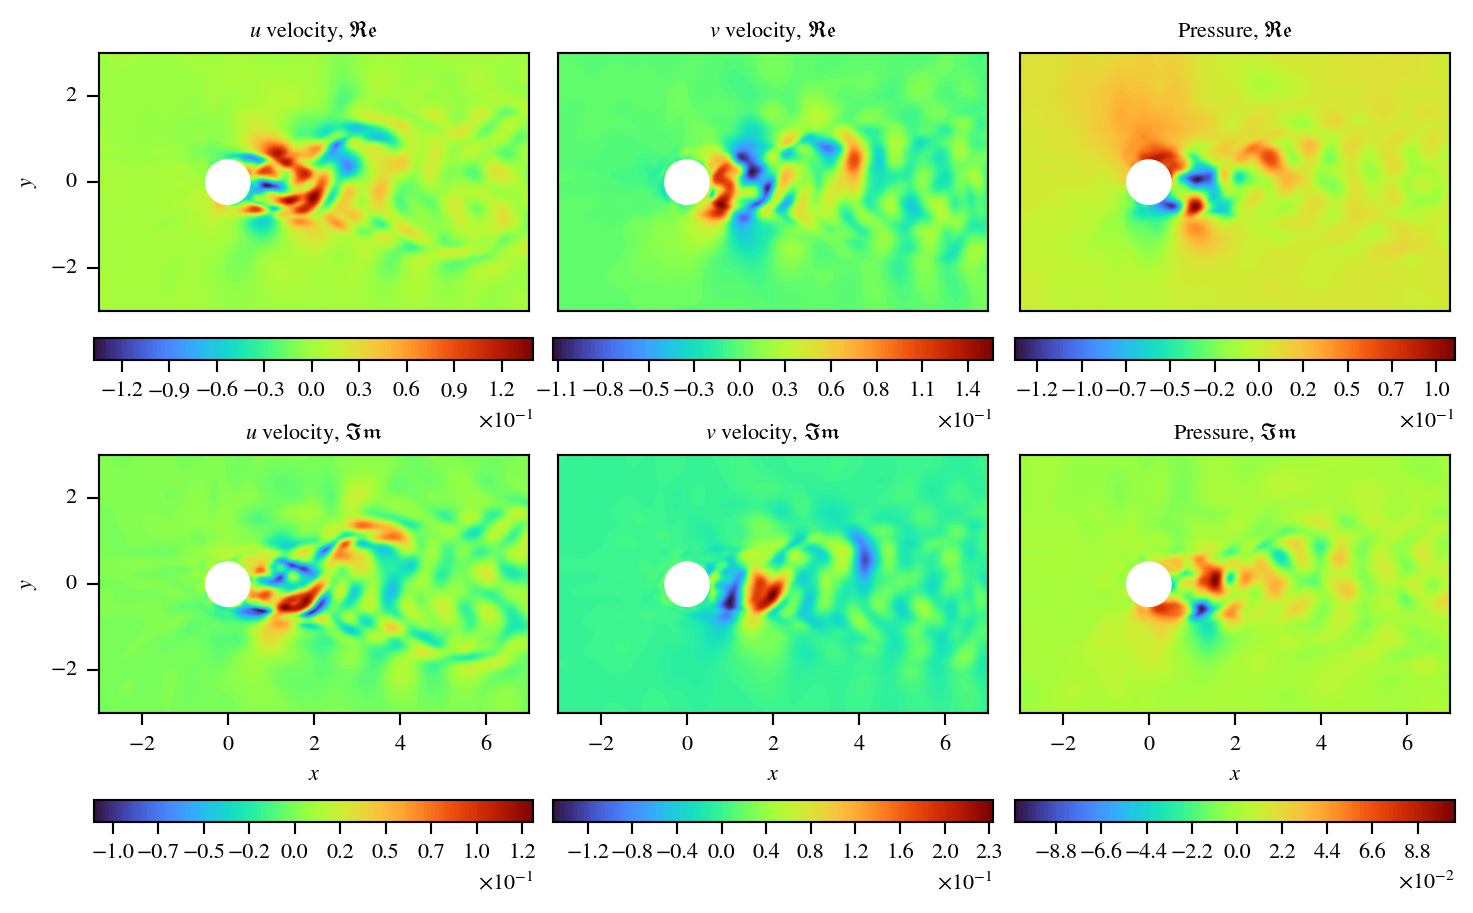
\includegraphics[width=0.95\textwidth]{cylinder-2d-re200/koopman_pinn_005_st0.761.png}%
    \caption{%
        The \num{4}th damped mode in data-driven PINN.
    }
    \label{fig:cylinder-re200-koopman-pinn-damped-4th}%
\end{figure*}

% vim:ft=tex: